Let $C$, $D $ be $3x\times 3$ matrices defining quadratic forms which cut out a general pair of conics in the projective plane. Let:
\[f(t)=\sqrt{\mathrm{det}(tC+D)}=\sum_{i=0}^\infty a_it^i=a_0+a_1t+a_2t^2+\cdots
 \]
 be the Taylor series of a branch of the square root of the cubic 
$\mathrm{det}(D+tC)$.
 Then there exists a Poncelet polygon, inscribed in 
$C$ and circumscribed about 
$D$, with vertex count dividing $n$
 if and only if the determinant of an associated 
$[\frac{n-1}{2}]$-dimensional Hankel matrix defined below vanishes. 
 {\small 
 \begin{align*}
     \left|\begin{matrix} a_2 &a_3 &\ldots & a_{p+1}\\
     a_3 & a_4&\ldots & a_{p+2}\\
     \ldots & \ldots & \ldots &\ldots\\
     a_{p+1}& a_{p+2}&\ldots & a_{2p}
     \end{matrix}\right|=0, n=2p+1, \mathrm{or}:\;\;  \left|\begin{matrix} a_3 &a_4 &\ldots & a_{p+1}\\
     a_4 & a_5&\ldots & a_{p+2}\\
     \ldots & \ldots & \ldots &\ldots\\
     a_{p+1}& a_{p+2}&\ldots & a_{2p-1}
     \end{matrix}\right|=0,\; n=2p.
 \end{align*}
 }
\section{Darboux theorem}

\begin{theorem}[\cite{darboux1917} ] Let $ S\subset \mathbb{P}_2$
  be a curve of degree $n-1$. If there is a complete $n-$gon tangent
to a smooth conic $C$ and inscribed into $S$, then there are infinitely many of them.
\label{th:darboux}
\end{theorem}
\begin{proof}
See \cite[Chapitre I, page 248]{darboux1917}.
\end{proof}
\begin{example}
Consider the cubic curve and the circle defined by
\[C_3(x,y)=-4x^2-5y^2+3x(y^2-1)+9=0,\; C(x,y)=x^2+y^2-1=0.\]
There is a porism of 4-periodic orbits (quadrilaterals) inscribed in the compact component of $C_3(x,y)=0$ and tangents to the circle  $C(x,y)=0.$ See \cref{fig:C3C2}.
In fact, the square with vertices $(\pm 1, \pm 1)$ is inscribed in $C_3(x,y)=0.$
\end{example}

\begin{figure}[H]
\begin{center}
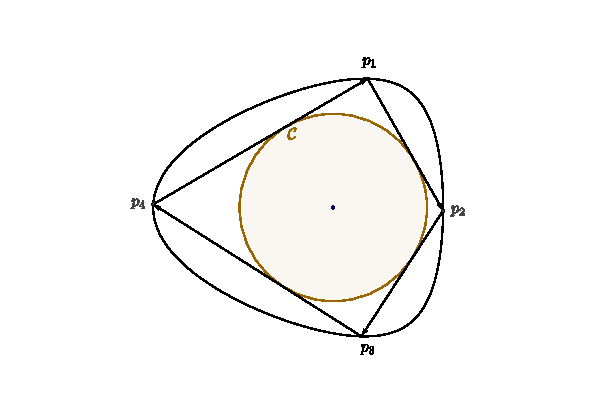
\includegraphics[scale=0.7]{chap_02/pics/pics_02_030_C3C2.pdf}
\end{center}
\caption{Porism of 4-periodic orbits associated to $C_3(x,y)=0$ and the unit circle. }
\label{fig:C3C2}
\end{figure}

Consider a pair of conics (ellipses) defined by two quadratic forms $q_1(x,y,z)=\frac{x^2}{a_1^2}+\frac{y^2}{b_1^2}-z^2=0$ and $q_2(x,y,z)=\frac{x^2}{a_2^2}+\frac{y^2}{b_2^2}-z^2=0$ in projective coordinates $[x:y:z]$.

Let $f(t)=\sqrt{{\text det} (q_1+tq_2)}$ where

\begin{align*}
 q_i= \left(\begin{matrix}\frac{1}{a_i^2} &0 &0 \\
0 &\frac{1}{b_i^2} &0\\
0 & 0 &-1
\end{matrix}\right)
\end{align*}
